\chapter{Fractional Control}

Fraction-order control, especially fractional-order PID control, is becoming increasingly popular. There are two main topics we will consider: using a controller that has fractional-order derivatives in it and controlling fractional-order systsems. Fractional-order PID is fairly self-evident. Both the I and D terms in the controller may have non-integer order, such that the control input to a system, $u(t)$ is given by
\begin{equation*}
  u(t) = k_p e(t) + k_I \tensor*[_0]\D{^{-\lambda}_t} e(t) + k_I \tensor*[_0]\D{^{\mu}_t} e(t)
\end{equation*}
where $e(t)$ is the error signal. If $\lambda$ and $\mu$ are both one, then this is what we normally would call PID control and if they are not one, it is what we call fractional PID control. 

It makes some sense that since for normal PID control we have the three gains to tune and for fractional PID we have five parameters, the three gains and the two fractional orders, that with more degrees of freedom we can often design a better controller. How to effectively tune five parameters is an issue. Furthermore, a drawback to fractional PID is that the controller needs to either compute or approximate the fractional terms, which can be expensive and therefore slow because they are non local. As such, there has been a lot of effort to determine good appriximations for the fractional controller terms that retain the benefit of fractional PID but are fast to compute.

Controls in general is primarly concerned with stability and performance. We will consider stability first.

\section{Stability of Fractional-Order Transfer Functions}

Many of the topics covered in undergraduate controls courses are ultimately considering stability. For an integer order transfer function
\begin{equation*}
  G(s) = \frac{s^m + a_1 s^{m-1} + \cdots + a_m}{b_0 s^n + b_1 s^{n-1} + \cdots + b_n}
\end{equation*}
solutions will have decaying exponential terms if and only if all the roots of the denominator have negative real part. Many of the usual tools in controls are essentially directed towards that. 
\begin{itemize}
  \item Constructing and analyzing the \emph{Routh array} is a means to determine the number of right half plane poles of the transfer function (but it does not fully factor the characteristic equation).
  \item The \emph{root locus} method is a way to plot how the pole locations of a transfer function change as some parameter in the system changes. It is especially useful when the transfer function is made up of interactions among relatively simple, \ie, factorable, sub-transfer functions with some feedback. Modern computational tools make it not particularly valuable as a means to simply determine the pole locations of a transfer function, \emph{but knowing how poles and zeros affect pole locations in a system provide valuable insighe into design controllers}.
  \item \emph{Bode plots} are a frequency-based tool that can provide insight into stability for a more limited class of systems (non-minimum phase), but are especially useful when a low-order model of a system is difficult to determine from first principles but the input-output behavior is relatively easy to determine experimentally.
  \item \emph{Nyquist plots} are also frequency-based with fewer restrictions than Bode plots.
\end{itemize}
An extremely important point that is always made, but often forgotten because all the work ever given in a controls course automatically satisfy it, is that the class of transfer functions for which such tools work are \emph{rational and proper}. Rational means they are ratios of polynomials (autmatically \emph{not} satisfied in the fractional case) and proper means that the order of the denominator is greater than the numerator.

In order to develop some convenient tools to study stability for fractional-order transfer functions, we first need to understand the asymptotic properties of the Mittag-Leffler functions, \ie, we know that in the integer-order case that poles with positive real parts correspond to terms in the solution with exponentials that increase in time, so what is the generalization of that to $\E_{\alpha,\beta}$?

\begin{theorem}
  For $0 < \alpha < 2$ and all $\beta$, 
  \begin{equation*}
    \lim_{ t \rightarrow \infty} \E_{\alpha,\beta} \left( a t \right) \approx \frac{1}{\alpha} t^{\frac{1-\beta}{\alpha}}\e^{\left( a t \right)^\frac{1}{\alpha}}.
  \end{equation*}
  \label{th:mlfasymptotics}
\end{theorem}

The proof is beyond the scope of this book, but see \cite{fraccontrol,mlfbook}. Here we can check this for a few different cases of $\alpha$, $\beta$ and $a$.

\begin{remark}
  For stability this theorem provides some easy boundaries:
  \begin{itemize}
  	\item If $a \in \mathbb R$, then we need $a < 0$ as usual.
  	\item If $a \in \mathbb C$, then we need the real part of $a$ to be negative as usual.
  	\item The value of $\beta$ does not matter.
	\item The theorem only applies for $0 < \alpha < 2$.
  \end{itemize}
  Note that as $\alpha \rightarrow 2$, the region in the complex plan where the poles must be for stability shrinks to nothing. In the case where $a \in \mathbb R$, this makes sense because the square root of a negative number is purly imaginary and cube roots will have a positive real part. When $a > 0$, one of the roots will always be positive.
\end{remark}

\begin{example} \hspace*{1in} \\
  \begin{enumerate}
    \item Figure~\ref{fig:mlfasyex1} plots $\E_{1,2}\left(-2 t \right)$ and the corresponding asymptotic expression from Theorem~\ref{th:mlfasymptotics}. 
    \item Figure~\ref{fig:mlfasyex2} plots $\E_{3/2,1/2}\left(-t \right)$ and the corresponding asymptotic expression from Theorem~\ref{th:mlfasymptotics}. 
    \item Figure~\ref{fig:mlfasyex3} plots $\E_{1,2}\left(t \right)$ and the corresponding asymptotic expression from Theorem~\ref{th:mlfasymptotics}. 
  \end{enumerate} 
\end{example}

\begin{figure}  
  \centering
  \subimport{figs/}{mlfasyex1}
  \caption{Mittag-Leffler function $\E_{1,2}\left(-2 t\right)$ (blue) and asymptotic approximation (red).}
  \label{fig:mlfasyex1}
\end{figure}

\begin{figure}  
  \centering
  \subimport{figs/}{mlfasyex2}
  \caption{Mittag-Leffler function $\E_{3/2,1/2}\left(-t\right)$ (blue) and asymptotic approximation (red).}
  \label{fig:mlfasyex2}
\end{figure}

\begin{figure}  
  \centering
  \subimport{figs/}{mlfasyex3}
  \caption{Mittag-Leffler function $\E_{1,2}\left(t\right)$ (blue) and asymptotic approximation (red).}
  \label{fig:mlfasyex3}
\end{figure}

Recall the main Laplace transform table entry for Mittag-Leffler functions:
\begin{equation*}
  \mathcal L \left\{ t^{\beta - 1} \E_{\alpha,\beta} \left( \pm a t^\alpha \right) \right\} = \frac{s^{\beta-\alpha}}{s^\alpha \mp a}.
\end{equation*}
The thing to note here is that the denominator term, $s^\alpha + a$ plays a very similar role as the integer-order poles we are used to considering. In other words, by inspection we can tell that a denominator $s-3$ corresponds to an unstable component of the solution and $s+2$ corresponds to a stable one. Theorem~\ref{th:mlfasymptotics} essentially verifies the same thing for a denominator term like $s^{1/2}+2$ in the fractional case as long as $0 < \alpha < 2$.

\begin{definition}
  A fractional transfer function is of the form
  \begin{equation*}
    G(s) = \frac{\sum_{k=1}^m b_k s^{\beta_k}}{\sum_{k=1}^n a_k s^{\alpha_k}}
  \end{equation*}
  where the $\alpha_k \geq 0$ are called the denominator orders and correspodingly the $\beta_k \geq 0$ are the numerator orders. 
  Often we will normalize it by requiring one of the coefficients to be zero, say $a_1=0$. 
  \label{def:fractionalxf}
\end{definition}

\subsection{Commensurable Transfer Functions}
A particularly convenient situation arises in the case of \emph{commensurable transfer functions}.

\begin{definition}
  A transfer function is said to be commensurable when all the orders $\alpha_k$ and $\beta_k$ are integer multiples of a common divisor $\alpha > 0$. In that case the transfer function is rational in $s^\alpha$. If we let $\lambda = s^\alpha$ then
  \begin{equation*}
    G(s) = \frac{\sum_{k=1}^m b_k s^{\beta_k}}{\sum_{k=1}^n a_k s^{\alpha_k}} = \frac{\sum_{k=0}^m b_k s^{\alpha k}}{\sum_{k=0}^n a_k s^{\alpha k}} = 
    \frac{\sum_{k=0}^m b_k \lambda^{k}}{\sum_{k=0}^n a_k \lambda^{k}}.
  \end{equation*}
  Of course, if all the coefficients of the numerator and denominatore are integer multiples of $\alpha$, they will also be integer multipes of $\alpha/2$, so it is convenient to chose the largest $\alpha$. 
  \label{def:commensurable}
\end{definition}

\begin{example}
  The transfer function
  \begin{equation*}
    G(s) = \frac{s + 3 s^\frac{1}{2} + 5}{s^2 + 2 s^\frac{3}{2} + s^\frac{1}{2} + 2}
  \end{equation*}
  is commensurable with $a = 1/2$ because if we let $\lambda = 1/2$
  \begin{equation*}
    G(s) = \frac{\lambda^2 + 3 \lambda + 5}{\lambda^4 + 2 \lambda^3 + \lambda + 2}.
  \end{equation*}
\end{example}

Stability of commensurable transfer functions has a transparent extension to integer-order transfer functions, but we first need to characterize the idea of left- and right-half planes slightly differently. Another way to say that all the poles of an integer-order transfer function must be in the left half of the complex plane is to require that the absolute value of the angle of the poles (as complex numbers) is greater than $\pi/2$, or more formally, we have the following theorem.

\begin{theorem}
  The commensurable transfer function
  \begin{equation*}
    G(s) =  \frac{\sum_{k=1}^m b_k s^{a k}}{\sum_{k=1}^n a_k s^{a k}} = 
    \frac{\sum_{k=1}^m b_k \lambda^{k}}{\sum_{k=1}^n a_k \lambda^{k}}
  \end{equation*}
  is stable if the solutions to $a_n \lambda^n + a_{n-1} \lambda^{n-1} + \cdots + a_0 = 0$, denoted by $\lambda_k$ are such that
  \begin{equation*}
    \left| \angle \lambda_k \right| > a \frac{\pi}{2}.
  \end{equation*}
  \label{th:commensurablestability}
\end{theorem}

\begin{proof}
  (for now follows very closely what is in \cite{fraccontrol}).

  If there are no repeated roots, then $G(s)$ can be written as the usual sort of partial fraction expansion
  \begin{equation*}
    G(s) = \sum_{k=1}^n \frac{\rho_k}{\lambda - \lambda_k} =  \sum_{k=1}^n \frac{\rho_k}{s^\alpha - \lambda_k}
  \end{equation*}
  so the impulse response will be of the form
  \begin{equation*}
    x(t) = \sum_{k=1}^n \rho_k t^{\alpha-1} \E_{\alpha,\alpha} \left( \lambda_k t^\alpha \right).
  \end{equation*}
  The asymptotic behavior of the solution is, as $t \rightarrow +\infty$
  \begin{equation*}
    x(t) \approx \sum_{k=1}^n \rho_k t^{\alpha-1} \frac{1}{\alpha} \left( \lambda_k t^\alpha \right)^\frac{1-\alpha}{\alpha} \e^{\left( \lambda_k t^\alpha \right)^\frac{1}{\alpha}} = \sum_{k=1}^n \frac{\rho_k}{\alpha}\lambda^{\frac{1-\alpha}{\alpha}}\e^{t \lambda_k^\frac{1}{\alpha}}.
  \end{equation*}
  This will be stable as long as the real part of $\lambda_k^{1/\alpha} < 0$. Since
  \begin{align*}
    \lambda_k^{1/\alpha} &= \left[ \left| \lambda_k \right| \left( \cos \angle \lambda_k + \iu \sin \angle \lambda_k \right) \right]^{1/\alpha} \\
    &= \left| \lambda_k \right|^{1/\alpha} \left( \cos \frac{\angle \lambda_k}{\alpha} + \iu \sin \frac{\angle \lambda_k}{\alpha} \right).
  \end{align*}
  The cosine term will be negative when its argument is greater than $\pi/2$, so we have
  \begin{equation*}
    \frac{\angle \lambda_k}{a} > \frac{\pi}{2}
  \end{equation*}
  or
  \begin{equation*}
    \angle \lambda_k > a \frac{\pi}{2}.
  \end{equation*}
  which is the desired result.
\end{proof}

\begin{remark}
  In the integer order case, $a = 1$ and the angle condition is the same as requiring all the poles to be in the left half plane.
\end{remark}

Consider the following program that uses the Gr\"unwald-Letnikov numerical approximation to numerically compute the solution to
\begin{equation*}
  \frac{\d x}{\d t}(t) + a \frac{d^\frac{1}{2} x}{\d t^\frac{1}{2}}(t) + b x(t) = 1
\end{equation*}
assuming all initial conditions of all orders are zero. Note that the \texttt{bincoeff()} function uses the \texttt{gammaln()} function to extend the domain over which it returns a non-zero value. We will use this program to compute numerical step responses for the next couple examples.

\lstinputlisting[language=matlab]{step.m}

\begin{example}
  Is the solution
  \begin{equation*}
  	\frac{\d x}{\d t}(t) -2  \frac{d^\frac{1}{2} x}{\d t^\frac{1}{2}}(t) + 5 x(t) = 1
  \end{equation*}
  where all initial conditions of all orders are zero stable?

  Since all initial conditions are zero, the Laplace transform of the equation is the same if we use the Riemann-Liouville or Caputo fractional derivatives, and we get
  \begin{equation*}
    X(s) = \frac{1}{s - 2 s^\frac{1}{2} + 5}.
  \end{equation*}
  This transfer function is commensurate of order $a = 1/2$ and will be stable of all roots of
  \begin{equation*}
    \lambda^2 - 2 \lambda + 5 = 0
  \end{equation*}
   are such that $\left| \angle \lambda_i \right| > \frac{1}{2} \frac{\pi}{2}$.  In this case $\lambda = 1 \pm 2 \iu$ which has an angle greater than $45^\circ$, so the system is stable. 

	A numerically-computed solution is in Figure~\ref{fig:comstableex1}.
	\label{ex:comstableex1}
\end{example}

\begin{figure}
  \centering
  \subimport{figs/}{comstableex1}
  \caption{Step response for Example~\ref{ex:comstableex1}.}
  \label{fig:comstableex1}
\end{figure}

\begin{example}
  Is the solution
  \begin{equation*}
  	\frac{\d x}{\d t}(t) -4  \frac{d^\frac{1}{2} x}{\d t^\frac{1}{2}}(t) + 5 x(t) = 1
  \end{equation*}
  where all initial conditions of all orders are zero stable?

  Since all initial conditions are zero, the Laplace transform of the equation is the same if we use the Riemann-Liouville or Caputo fractional derivatives, and we get
  \begin{equation*}
    X(s) = \frac{1}{s - 4 s^\frac{1}{2} + 5}.
  \end{equation*}
  This transfer function is commensurate of order $a = 1/2$ and will be stable of all roots of
  \begin{equation*}
    \lambda^2 - 4 \lambda + 5 = 0
  \end{equation*}
   are such that $\left| \angle \lambda_i \right| > \frac{1}{2} \frac{\pi}{2}$.  In this case $\lambda = 2 \pm  \iu$ which has an angle less than $45^\circ$, so the system is unstable. 

	A numerically-computed solution is in Figure~\ref{fig:comstableex2}.
	\label{ex:comstableex2}
\end{example}

\begin{figure}
  \centering
  \subimport{figs/}{comstableex2}
  \caption{Step response for Example~\ref{ex:comstableex2}.}
  \label{fig:comstableex2}
\end{figure}

Because we normally do not factor separate complex terms, it makes sense to consider stability of a ``second-order'' type commensurable system. Analogous to the ubiquitous $\omega_n^2/\left( s^2 + 2 \zeta \omega_n s + \omega_n^2 \right)$ transfer function, consider
\begin{align}
  G(s) &= \frac{k}{m s^{2 \alpha} + b s^\alpha + k} \nonumber \\
  &= \frac{\omega_n^2}{s^{2 \alpha} + 2 \zeta \omega_n s^\alpha + \omega_n^2} \nonumber \\
  &= \frac{1}{\left( \frac{s^\alpha}{\omega_n} \right)^2 + 2 \zeta \left( \frac{s^\alpha}{\omega_n} \right) + 1}. \label{eq:secondcommensurable}
\end{align}

The solutions of $\lambda^2/\omega_n^2 + 2 \zeta \lambda/\omega_n + 1 = 0$ are
\begin{equation*}
  \lambda = \omega_n \left( -\zeta \pm \sqrt{\zeta^2-1} \right) \qquad \Longleftrightarrow \qquad
  s^\alpha =  \omega_n \left( -\zeta \pm \sqrt{\zeta^2-1} \right).   
\end{equation*}
From this we can infer the following:
\begin{enumerate}
  \item If $\zeta > 1$ both roots are real and both are negative. Hence the transfer function is stable as long as $0 < \alpha < 2$
  \item  If $\zeta < -1$, then at least one root is positive and hence the transfer function is unstable.
  \item If $\zeta = 0$, then the roots are $\pm \iu \omega_n$. Hence the transfer function will be stable if $\alpha < 1$ and unstable if $\alpha > 1$. 
  \item If $0 < \zeta < 1$ and $0 < \alpha \leq 1$, then the roots are complex with negative real part. Since $\alpha < \leq 1$ the entire left half plane is in the stability region and hence the transfer function is stable.
  \item If $-1 < \zeta < 0$ and $0 < \alpha < 1$, then the roots are complex with a positive real part. To be stable, $\alpha$ must be small enough so that the roots are in the stability region. The tangent of the angle is given by the ratio of the imagainary to the real part of the pole, so for stability we require 
    \begin{equation*}
      \tan^{-1} \frac{\sqrt{1 - \zeta^2}}{-\zeta} > \alpha \frac{\pi}{2} \quad \Longrightarrow 
      \frac{\sqrt{1 - \zeta^2}}{-\zeta} > \tan \frac{\alpha \pi}{2}.
    \end{equation*}
    Because $\zeta < 0$ the left hand side is positive 
    \begin{equation*}
      \frac{1 - \zeta^2}{\zeta^2} > \tan^2 \frac{\alpha \pi}{2} \qquad \Longleftrightarrow \qquad
      \cos^2 \frac{\alpha \pi}{2} > \zeta^2.
    \end{equation*}
    Because $\zeta < 0$, we finally have that the transfer function is stable if
    \begin{equation*}
      \zeta > -\cos \frac{\alpha \pi}{2}.
    \end{equation*}
  \item A similar argument shows that if $0 < \zeta < 1$ and $1 < \alpha < 2$, the transfer function is stable if 
    \begin{equation*}
      \zeta > -\cos \frac{\alpha \pi}{2}.
    \end{equation*}
  \item Finally, if $-1 < \zeta < 0$ and $1 \leq \alpha < 2$ the roots are complex and in the right half plane. Because $\alpha > 1$ the stability region is ``less than'' the left half plane. Hence the transfer function is always unstable.
\end{enumerate}

Figure~\ref{fig:secondstable} illustrates the stability regions for a commensurable transfer fuction where the area above the curve is stable and the area under the curve is unstable.

\begin{figure}
  \centering
  \subimport{figs/}{secondstable}
  \caption{Stability regions for transfer functions of the form given by Equation~\ref{eq:secondcommensurable}.}
  \label{fig:secondstable}
\end{figure}

\section{Frequency Response}
Bode plots for fractional-order systems are computationally straight-forward to construct by simply defining set of discrete frequencies and evaluating $\left| G \left( \iu \omega \right) \right|$ and $\angle G \left( \iu \omega \right)$ at those frequencies. 

\begin{example}
  Consider
  \begin{equation}
    G(s) = \frac{1}{s^\frac{1}{2} + 10}.
    \label{eq:fracfreqex1}
  \end{equation}
  The Bode plot for that transfer function is illustrated in Figure~\ref{fig:fracfreqex1}.

  Observe that for high frequencies the slope of the magnitude curve is $-10$db/decade and the phase is $-45^\circ$.

  The code that generated Figure~\ref{fig:fracfreqex1} is:

\lstinputlisting[language=matlab]{freq.m}
\end{example}

\begin{figure}
  \centering
  \subimport{figs/}{fracfreqex1}
  \caption{Frequency response for system in Equation~\ref{eq:fracfreqex1}.}
  \label{fig:fracfreqex1}
\end{figure}

\section{Integer-Order Approximations for Fractional-Order Transfer Functions}
It may be the case that we want to use an integer-order transfer function that mimics a fractional order one. That could be, for example, if we design a fractional-order controller. In that case, when we implement the controller we may use an integer-order approximation that has approximately the same dynamics.

Recall that the way to draw the magnitude plot for
\begin{equation*}
  G(s)= \frac{p}{s+p}
\end{equation*}
the usual approach is to treat the magnitude as $0$dB for frequencies less than $p$ and then for frequencies greater than $p$, as a line with a slope of $-20$dB/decade (on a log-dB scale). So, when the frequency crosses from a lower to higher frequency than a pole, the slope decreases by $20$dB/decade. Correspondingly when the frequency crosses a zero, the slope increases by $20$dB/decade. Thus if we properly space poles and zeros we can construct a stair-case type magnitude plot that, on average, has a slope of, say, $-10$dB/decade. In fact, if the poles are evenly spaced logarithmically with the zeros half way between each pole (again logarithmically), we would expect a slope of $-10$dB/decade. Analogous reasoning will lead to a phase of $-45^\circ$.

\begin{example}
  Consider 
  \begin{equation}
    G(s) = \frac{ \left(s + 0.0316 \right) \left(s + 0.316 \right)  \left(s + 3.16 \right) \left(s + 31.6 \right)  
    }{\left(s+0.01 \right)\left(s+0.1 \right) \left(s+1 \right) \left(s+10 \right) \left(s+100 \right)} 
    \label{eq:PID}
  \end{equation}
\end{example}

\section{Fractional-Order PID}
As mentioned at the beginning of this chapter, we can generalize PID control to the fractional case by allowing the derivative and integral terms to have a fractional order, \ie, 
\begin{equation*}
  u(t) = k_p e(t) + k_I \tensor*[_0]\D{^{-\lambda}_t} e(t) + k_I \tensor*[_0]\D{^{\mu}_t} e(t)
\end{equation*}
where $u(t)$ is the input and $e(t)$ is the error signal. Fractional-order PID should generally allow for better performance because integer-order PID is among the options available, \ie, the special case where we choose $\lambda = \mu = 1$. However, we do need a method to search for all five parameters. The main benefit of PID control, and hence its ubiquity, is that it is fairly straight-forward to tune on a real system. In other words, we do not need a mathematical model to design the controller if the approach is to implement PID in hardware and tune the three gains by experiment on the real system. Specifically, for a second-order plant, the three gains have very straight-forward effects: increasing the proporational gain increases the natural frequency, increasing the derivative gain increases the damping and increasing the integral gain decreases the time to eliminate steady-state error.

In this chapter we take an alternative approach when a good mathematical model is avaiable, which is to implement an optimization algorithm to search for the best gains. Because optimization is not generally covered in many controls courses, first we will present a problem implementing this in full detail.

\subsection{Optimization of a PID Controller}
The example in this section is taken from \cite{YQChenAcc}. Consider a DC motor driving a load as illustrated in Figure~\ref{fig:PIDex}. An input voltage drives a circuit with a dc motor. The motor shaft has an inertia $J_m$ and its motion is resisted by viscous friction described by the coefficient $\beta_m$. The angle of the motor shaft is given by $\theta_m$. The shaft is attached to a gearbox with a gear ratio of $\rho$, and the output of the gear box drives the load. The inertia of the load is $J_L$ and the motion of the load is resisted by viscous friction with a coefficient of $\beta_L$. The shaft connecting the output of the gearbox to the load is flexible and acts like a torsional spring with spring constant $k_\theta$. 

\begin{figure}
  \centering
  \psfrag{R}{$R$}
  \psfrag{V}{$V_{in}$}
  \psfrag{qm}{$\theta_m$}
  \psfrag{ql}{$\theta_L$}
  \psfrag{Jm}{$J_m, \beta_m$}
  \psfrag{Jl}{$J_L, \beta_L$}
  \psfrag{r}{$\rho$}
  \psfrag{kt}{$k_\tau, k_e$}
  \psfrag{kth}{$k_\theta$}
  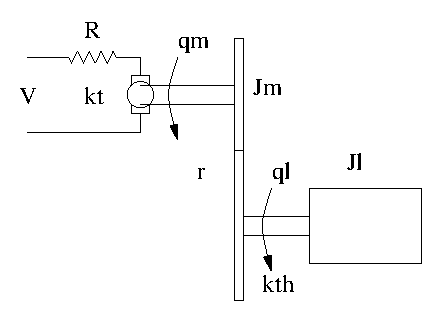
\includegraphics{figs/PIDex}
  \caption{PID system.}
  \label{fig:PIDex}
\end{figure}

\textbf{Problem Statement:} Use PID control given by Equation~\ref{eq:PID} where $u(t)$ is the voltage into the circuit and $e(t)$ is the difference between the desired angle of the load and the actual angle of the load. Find the optimal gains, $k_p$, $k_d$ and $k_i$ such that:
\begin{itemize}
  \item The cost function
    \begin{equation}
      J = \int_0^{60} \left( \theta_{desired}(t) - \theta_L(t) \right)^2 \d t 
      \label{eq:optcf}
    \end{equation}
    is minimized;
  \item $\left| V_{in}(t) \right| \leq 220$ 
  \item The torque in the output shaft of the gearbox driving the load always has a magnitude less than $100$Nm.
\end{itemize}
This is a \emph{constrained optmization problem}. We will use the Matlab function \texttt{fmincon()} to find a solution.

Kirchhoff's voltage law gives
\begin{equation*}
  V_{in}(t) = i(t) R + k_e \dot \theta_m(t)
\end{equation*}
where $i(t)$ is the current through the motor. Hence, the output torque from the motor is given by
\begin{equation*}
  \tau_m(t) = k_\tau \left( \frac{V_{in}(t) - k_e \dot \theta_m(t)}{R} \right).
\end{equation*}
Newton's law on the motor shaft is given by
\begin{equation*}
  J_m \ddot \theta_m(t) = k_\tau \left( \frac{V_{in}(t) - k_e \dot \theta_m(t)}{R} \right) - \beta_m \dot \theta_m(t) + \frac{k_\theta}{\rho} \left( \theta_L(t) - \frac{\theta_m(t)}{\rho} \right)
\end{equation*}
and similarly on the load
\begin{equation*}
  J_l \ddot \theta_L(t) = -k_\theta \left( \theta_L(t) - \frac{\theta_m(t)}{\rho} \right) - \beta_L \dot \theta_L(t).
\end{equation*}

If we define the state vector as
\begin{equation*}
  x(t) = \begin{bmatrix} \theta_L(t) \\ \dot \theta_L(t) \\ \theta_m(t) \\ \dot \theta_m(t) \end{bmatrix}
\end{equation*}
then we can express the equations of motion in the standard state space form of $\dot x(t) = A x(t) + B V_{in}(t)$ as
\begin{equation}
  \frac{\d}{\d t} \begin{bmatrix} \theta_L(t) \\ \dot \theta_L(t) \\ \theta_m(t) \\ \dot \theta_m(t) \end{bmatrix} =
  \begin{bmatrix}
	0 & 1 & 0 & 1 \\
	-\frac{k_\theta}{J_L} & -\frac{\beta_L}{J_L} & \frac{k_\theta}{\rho J_L} & 0 \\
	0 & 0 & 0 & 1 \\
	\frac{k_\theta}{\rho J_m} & 0 & -\frac{k_\theta}{\rho^2 J_m} & - \left( \frac{k_\tau k_e}{J_m R} + \frac{\beta_M}{J_m} \right)
  \end{bmatrix}
  \begin{bmatrix}
    \theta_L(t) \\ \dot \theta_L(t) \\ \theta_m(t) \\ \dot \theta_m(t)
  \end{bmatrix}
  + 
  \begin{bmatrix}
    0 \\ 0 \\ 0 \\ \frac{k_\tau}{J_m R}
  \end{bmatrix} V_{in}(t).
  \label{eq:PIDexeom}
\end{equation}
If the only state we can measure is $\theta_L(t)$ then in the standard form $y(t) = C x(t) + D V_{in}(t)$ we have
\begin{equation*}
  y = \begin{bmatrix} 1 & 0 & 0 & 0 \end{bmatrix} x(t).
\end{equation*}

From~\cite{YQChenAcc} let 
\begin{itemize}
  \item $k_\theta = 1280.2$
  \item $k_\tau = 10$
  \item $k_e = 10$ 
  \item $J_m = 0.5$ 
  \item $J_L = 25$
  \item $\rho = 20$
  \item $\beta_m = 0.1$
  \item $\beta_L = 25$
  \item $R = 20$.
\end{itemize}
Using those values and constructing $A$, $B$, $C$ and $D$ in Matlab, and then using \texttt{G = ss2tf(A,B,C,D)} gives the transfer function from the input voltage to the angular position of the load as
\begin{equation*}
  G(s) = \frac{\Theta_L(s)}{V_{in}(s)} = \frac{2.56}{s^4 + 11.2 s^3 + 67.81 s^2 + 528.7 s}
\end{equation*}
which is a type 1 system, which also makes sense.

If we already have PID gains, or we wish to tune the controller by hand, then we can use set numerical values for the gains and use \texttt{Con = tf([kd + kp + ki],[1 0])} to define the PID controller transfer function, from which \texttt{step(feedback(Con*G,1))} will plot the step response. 

Because our goal is to compare integer-order PID control with fractional-order PID control, we need an objective basis for comparison. As such, we will set up an optimization problem to find the ``best'' PID gains in each case, and compare the results. We will use \texttt{(fmincon()} in Matlab. From the documentation, the function attempts to find the minimum of a problem specified by
\begin{equation}
  \min_x f(x) \mbox{such that} \begin{cases} c(x) &\leq 0 \\ 
    c_{eq}(x) &= 0 \\ 
					A x &\leq b \\ 
					A_{eq} x &= b_{eq} \\ 
					lb &\leq x \leq ub  \end{cases}
  \label{eq:opt}
\end{equation}
For the constraints
\begin{itemize}
  \item $c(x) \leq 0$ are the nonlinear inequality constraints
  \item $c_{eq}(x) = 0$ are the nonlinear equality constraints
  \item $Ax \leq b$ are the linear inequality constraints
  \item $A_{eq} x = b_{eq}$ are the linear equality constraints
  \item $lb \leq x \leq ub$ are the bound constraints.
\end{itemize}
The Matlab syntax is
\begin{center}
  \texttt{fmincon(fun,x0,A,b,Aeq,beq,lb,ub,nonlin)}
\end{center}
where 
\begin{itemize}
  \item \texttt{fun} is the function to be minimized
  \item \texttt{x0} is the initial guess for the solution
  \item \texttt{A} is the matrix in the linear inequality constraints
  \item \texttt{b} is the right hand side of the linear inequality consntraints
  \item \texttt{Aeq} is the matrix in the linear equality constraints
  \item \texttt{beq} is the right hand side of the linear equality constraints
  \item \texttt{lb} and \texttt{ub} are the lower and upper bounds of the search space
  \item \texttt{nonlin} is the function of the nonlinear inequality and equality constraints (the are combined!).
\end{itemize}

For our problem, the function to be minimixed is given by Equation~\ref{eq:optcf}. Note that we are searching for optimal gains, so the gains are represented by $x$ in the previous equations describing \texttt{fmincon()}, which of course can be confusing because we are using $x$ to represent the states in our problem. We need a matlab function that evaluates Equation~\ref{eq:optcf}. So the function has to determine the step response for the given gains, and then compute the integral of the square of the difference between the desired angle and actual angle of the load.

So the function will have to call either \texttt{step()} or \texttt{ode45()} to compute the step response. With some foresight knowing we will have to compute the input voltage and the torque in the flexible shaft, we will solve the problem in state space using \texttt{ode45()}. The function (\texttt{sossserr()} ``sum of squares for the state space system of the error'') will need to know the equations of motion, time and the gains:

\begin{lstlisting}
function ret = sossserr(ks,A,B,C,D,t)
    [t,y] = ode45(@(t,x)sspidrhs(t,x,ks,A,B,C,D),t,[0; 0; 0; 0; 0]);
    ret = trapz(((1-y(:,1)).^2)*(t(2)-t(1)));
end
\end{lstlisting}

The right hand side of the differential equations needs an additional state appended to be able to compute the integral of the error. So a fifth state which is the integral of the error is appended, so its derivative is simply the error:

\begin{lstlisting}
function xdot = sspidrhs(t,x,ks,A,B,C,D)
    error = 1 - x(1);
    errordot = 0 - x(2);
    input = ks(1)*error + ks(2)*errordot + ks(3)*x(5);
    xdot(1:4) = A*x(1:4)+B*input;
    xdot(5) = error;
    xdot = xdot';
end
\end{lstlisting}

Using these functions, we now can find the best PID gains to minimize the integral of the square of the error. However, if we simply try to minimize $J$, then the algorithm to determine the gains will not coverge because arbitrarily high gains will drive the solution to the desired value of one. Hence, we must add bounds to the search using \texttt{lb} and \texttt{ub} or add in some other constraints. The real constraints are the voltage and torque limits, but because those are relatively difficult to implement, for now we will just put bounds on the allowable gain values.

